\section{Six Bar Cosmic-Ray Method}

The six bar cosmic-ray method is a generalization and improvement of
the three bar cosmic-ray method facilitating individual counter
resolution measurements.  As such, it is necessary to recapitulate the
three bar cosmic-ray method prior to presenting the six bar cosmic-ray
method.

\subsection{Three Bar Cosmic-Ray Method}
\label{sect:Three_Bar_Cosmic_Ray_Method}

The three bar cosmic-ray method (hereafter known as the three bar
method) allows the determination of the time resolution of a counter
given two counters with known time resolutions.  A counter here is a
scintillator with photomultiplier tubes (PMTs) attached at each end.
The three bar cosmic-ray method proceeds by stacking the three
counters vertically with equal spacing between adjacent counters and
each counter being parallel to the other two.

\begin{figure}[H]
  \centering
  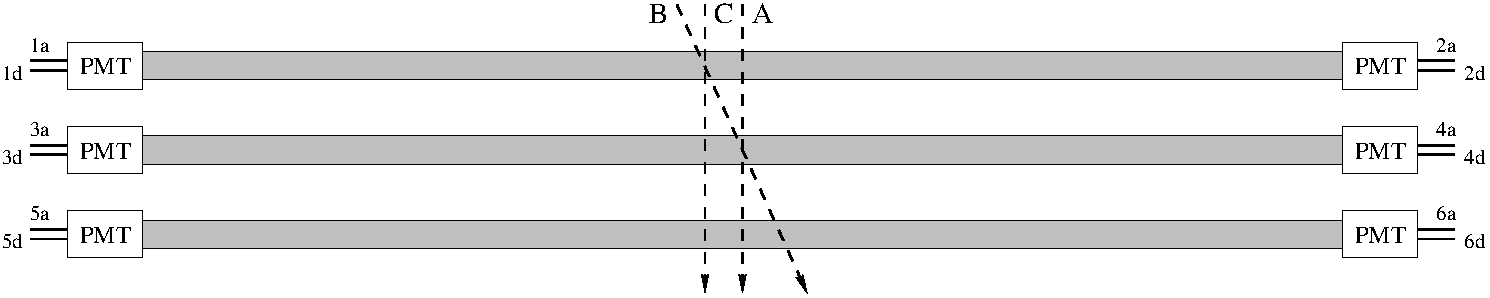
\includegraphics[width=15cm]{gary/fig_gary_three_bar/Fig14-M.pdf}
  \caption{In the three bar method, cosmic-ray particles are required
    to pass through all three counters.  A, B, and C denote possible
    particle paths through the three counters.}
  \label{3bar}
\end{figure}

%% This figure was deprecated due to earlier (and better) figure for
%% the three bar setup

%% \begin{figure}[H]
%%   \centering
%%   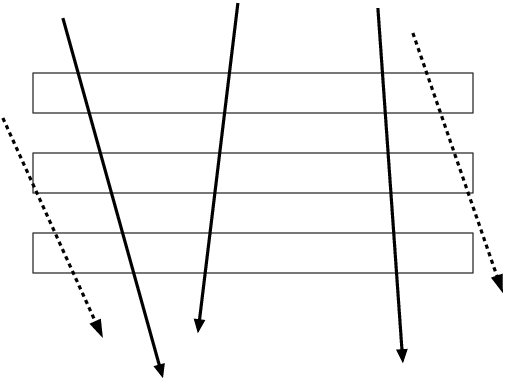
\includegraphics[width=15cm]{3bar.png}
%%   \caption{In the three bar method, cosmic-ray particles are required
%%     to pass through all three counters; solid lines illustrate
%%     detected particle tracks whereas dashed lines show discarded
%%     paths.}
%%   \label{3bar}
%% \end{figure}

Cosmic-ray particles will interact with the counters at random.  If
only those events in which all three counters detected a cosmic-ray
particle are considered, then the geometry of the setup allows the
unknown resolution to be determined.  The detected cosmic-ray
particles are assumed to have high enough energy so that the paths
they take are straight to good approximation (a good assumption in
practice).  Since the counters are arranged to be parallel with equal
spacing, and since the particle travels with fixed velocity, the time
taken to travel between any pair of adjacent counters is the same.

The interacting cosmic-ray particle causes each PMT to signal; these
are sent to a time-to-digital converter (TDC) and reported as the
interaction time of the scintillation light with the PMT.  One of the
six PMTs is chosen to provide the reference time for the event
\(t_{ref}\).  The reference time is subtracted from the raw time
reported from the TDC for each PMT since the raw TDC reported times
have arbitrary offsets.  Therefore the reference-subtracted timing for
each PMT is given by \(t = t_{\mathrm{raw}} - t_{ref}\).

The time that the cosmic-ray particle interacts with the
\(i\mathrm{th}\) scintillator is given by

\[t'_i = \frac{t_{iL} + t_{iR}}{2} - \frac{L}{2 v}\]

where \(t_{iL}\) and \(t_{iR}\) are the left and right PMTs for the
scintillator respectively, \(L\) is the length of the scintillator,
and \(v\) is the effective speed of light of the scintillator.
%% Not sure if this is right:
%% Since the PMT response depends on the amplitude of the light
%% received, \(v\) depends on both the material and geometry of the
%% scintillator.

However, since the counters have the same geometry and are made of the
same material, the counter term \(-\frac{L}{2 v}\) is the same for each
counter and can be subtracted from each counter interaction time to
yield
\[t_i = t'_i + \frac{L}{2 v} = \frac{t_{iL} + t_{iR}}{2}.\]
The counter interaction times for each of the three counters should be
given by:
\[t_{\mathrm{t}} = \tau + \varepsilon_{\mathrm{t}},\]
\[t_{\mathrm{m}} = \tau + \varepsilon_{\mathrm{m}} + \delta,\]
and
\[t_{\mathrm{b}} = \tau + \varepsilon_{\mathrm{b}} + 2 \delta,\]
where the \(t_i\) are the measured interaction times reported by the
electronics for each counter (top, middle, and bottom), \(\tau\) is
the actual time at which the cosmic-ray particle interacts with the
top counter, the \(\varepsilon_i\) are all the error contributions to
the measured time including those due to the electronics as well as
the intrinsic random contributions, and \(\delta\) is the time it
takes the cosmic-ray particle to move between adjacent counters.  As
noted above, this time \(\delta\) is the same for any pair of adjacent
counters due to equal spacing and the straight trajectory of the
cosmic-ray particle.

Note that the quantity
\[T = \frac{t_{\mathrm{t}}+t_{\mathrm{b}}}{2} - t_{\mathrm{m}} = \frac{\varepsilon_{\mathrm{t}}+\varepsilon_{\mathrm{b}}}{2} - \varepsilon_{\mathrm{m}}\]
does not depend on \(\tau\) or \(\delta\).  Since the resolution of
the readout electronics is typically small compared to the statistical
uncertainty in \(T\), the statistical uncertainty in \(T\) only
depends on the resolutions of the three counters:
\[\sigma_T^2 =
(\sigma_{\varepsilon_{\mathrm{t}}}^2+\sigma_{\varepsilon_{\mathrm{b}}}^2)/4+\sigma_{\varepsilon_{\mathrm{m}}}^2\]
where the \(\sigma_{\varepsilon_i}\) are the statistical
resolutions of the individual counters.  The assumption of identical
counters, $\forall i \; \sigma_{\varepsilon_i} = \sigma_{\varepsilon}$,
implies finally that

\[\sigma_T^2 = \frac{3}{2} \sigma_\varepsilon^2\]

or, rearranging,

\[\sigma_\varepsilon = \sqrt{\frac{2}{3}} \sigma_T\]
